\documentclass[../main.tex]{subfiles}
\graphicspath{{\subfix{../images/}}}
\begin{document}

\subsection*{Answers - Differential equations (page \pageref{Differential equations})}
\label{Differential equations answers}
\begin{spacing}{1.5}
\begin{enumerate}[itemsep=0.7cm]
    \item 
    \begin{enumerate}[itemsep=0.5cm]
        \item
        
        $\frac{dP}{dt}=\frac{1}{20}P(2P-1)\cos{t}$

        $\frac{1}{P(2P-1)}\,dP=\frac{1}{20}\cos{t}\,dt$

        $\int \frac{1}{P(2P-1)}\,dP=\int \frac{1}{20}\cos{t}\,dt$

        We need to use partial fractions for the left-hand side.

        $\frac{1}{P(2P-1)}=\frac{A}{P}+\frac{B}{2P-1}$

        $1=A(2P-1)+BP$

        $1=2AP-A+BP$

        $-A=1 \Rightarrow A=-1$

        $-2+B=0 \Rightarrow B=2$

        $\frac{1}{P(2P-1)}=-\frac{1}{P}+\frac{2}{2P-1}$

        Integrating:

        $\int \frac{2}{2P-1}-\frac{1}{P}\,dP=\int \frac{1}{20}\cos{t}\,dt$

        $\ln|2P-1|-\ln|P|=\frac{1}{20}\sin{t}+c$

        $\ln|\frac{2P-1}{P}|=\frac{1}{20}\sin{t}+c$

        $\frac{2P-1}{P}=Ae^{\frac{1}{20}\sin{t}}$

        Rearranging to make P the subject:

        $2P-1=APe^{\frac{1}{20}\sin{t}}$

        $2P-APe^{\frac{1}{20}\sin{t}}=1$

        $P(2-Ae^{\frac{1}{20}\sin{t}})=1$

        $P=\frac{1}{2-Ae^{\frac{1}{20}\sin{t}}}$

        Substituting $P=8$ when $t=0$:

        $8=\frac{1}{2-A}$

        $16-8A=1$

        $8A=15$

        $A=\frac{15}{8}$

        The model is:

        $P=\frac{1}{2-\frac{15}{8}e^{\frac{1}{20}\sin{t}}}$

        Multiplying by $\frac{8}{8}$ gives us:

        $P=\frac{8}{16-15e^{\frac{1}{20}\sin{t}}}$ as required.

        \item
        We know $-1\leq \sin{t} \leq 1$, so by substituting -1 and 1 into our model we will get the maximum and minimum populations.

        $\sin{t}=1$

        $P=\frac{8}{16-15e^{\frac{1}{20}}}=34.642 = 34,642$

        $\sin{t}=-1$

        $P=\frac{8}{16-15e^{-\frac{1}{20}}}=4.62 = 4,620$

        So the maximum is 34,642 and the minimum is 4,620.

        
    \end{enumerate}

    \item 
    \begin{enumerate}[itemsep=0.5cm]
        \item 
        $\frac{dh}{dt}=\frac{3}{2}\sqrt{h}\sin{\Bigl(\frac{3t}{4}\Bigr)}$

        $\frac{1}{\sqrt{h}}\,dh=\frac{3}{2}\sin{\Bigl(\frac{3t}{4}\Bigr)}\,dt$

        $\int \frac{1}{\sqrt{h}}\,dh=\int \frac{3}{2}\sin{\Bigl(\frac{3t}{4}\Bigr)}\,dt$

        $2\sqrt{h}=-2\cos{\Bigl(\frac{3t}{4}\Bigr)}+c$

        $\sqrt{h}=-\cos{\Bigl(\frac{3t}{4}\Bigr)}+c$

        Substituting in $t=0, h=1$:

        $1=-\cos{0}+c$

        $1=-1+c$

        $c=2$

        So the model is $\sqrt{h}=2-\cos{\Bigl(\frac{3t}{4}\Bigr)}$ as required.

        \item 
        We know that $-1 \leq \cos{\Bigl(\frac{3t}{4}\Bigr)}\leq 1$, which also means $-1 \leq -\cos{\Bigl(\frac{3t}{4}\Bigr)}\leq 1$.

        Therefore, we can add 2 to get $1 \leq 2-\cos{\Bigl(\frac{3t}{4}\Bigr)}\leq 3$

        Substituting $\sqrt{h}$:

        $1 \leq \sqrt{h} \leq 3$

        $1 \leq h \leq 9$

        Which means that the maximum height of the car is 9m.

        \item 
        $\sqrt{8}=2-\cos{\Bigl(\frac{3t}{4}\Bigr)}$

        $\cos{\Bigl(\frac{3t}{4}\Bigr)}=2-\sqrt{8}$

        $\frac{3t}{4}=\cos^{-1}(2-\sqrt{8})=2.547$

        Using the general formula for cosine:

        $\frac{3t}{4}=2n\pi \pm 2.547$

        $t=\frac{8n\pi}{3}\pm 3.396$

        Trying values of $n$:

        $n=0 : t=3.396$

        $n=1 : t=4.98$

        $n=2 : t=11.77$

        Therefore, the third time the car reaches 8m is at 11.77 seconds.

    \end{enumerate}

    \item 
    \begin{enumerate}[itemsep=0.7cm]
        \item 
        $\frac{dx}{dt}=-4\sin{t}-3\cos{t}$

        $\frac{dy}{dt}=-3\sin{t}+4\cos{t}$

        $\frac{dy}{dx}=\frac{dy}{dt}\times \frac{dt}{dx}=\frac{-3\sin{t}+4\cos{t}}{-4\sin{t}-3\cos{t}}=\frac{-3\sin{t}+4\cos{t}}{-(-4\sin{t}-3\cos{t})}$

        Since $x=4\cos{t}-3\sin{t}+1$, we know that $x-1=4\cos{t}-3\sin{t}$

        Since $y=3\cos{t}+4\sin{t}-1$, we know that $-y=-(3\cos{t}+4\sin{t})+1$, and therefore $-1-y=-(3\cos{t}+4\sin{t})$

        This means we have $\frac{dy}{dx}=\frac{x-1}{-1-y}=\frac{1-x}{1+y}$ as required.

        \item 
        Separate variables and integrate:

        $\int (1+y)\,dy=\int (1-x)\,dx$

        $y+\frac{y^2}{2}=x-\frac{x^2}{2}+c$

        $2y+y^2=2x-x^2+C$

        Applying the condition of $(5,2)$:

        $2(2)-(2)^2=2(5)-(5)^2+C$

        $C=23$

        The model is $2y+y^2=2x-x^2+23$

        Finding $y$ when $x=2$:

        $2y+y^2=23$

        $y^2+2y-23=0$

        $y=\frac{-2 \pm \sqrt{96}}{2}=-1 \pm 2\sqrt{6}$
    
    \end{enumerate}

    \item 
    \begin{enumerate}[itemsep=0.7cm]
        \item 
        $\frac{dx}{dt}=k(8-t)\times \frac{1}{x}$

        (Where $k$ is the proportion constant, $8-t$ represents the direct proportion to time left, and $\frac{1}{x}$ is inversely proportional to sales made)
   
        $\frac{dx}{dt}=\frac{k(8-t)}{x}$

        When $t=2, x=336, \frac{dx}{dt}=72$

        $72=\frac{k(8-2)}{336}$

        $k=4032$

        So, the model is $\frac{dx}{dt}=\frac{4032(8-t)}{x}$, which can be rearranged to $x\frac{dx}{dt}=4032(8-t)$

        \item 
        Separate variables and integrate:

        $\int x\,dx=4032\int (8-t)\,dt$

        $\frac{x^2}{2}=4032(8t-\frac{t^2}{2})+c$

        $x^2=4032(16t-t^2)+C$

        When $t=2, x=336$:

        $336^2=4032(16(2)-(2)^2)+C$

        $C=0$

        The model is $x^2=4032(16t-t^2)$

        \item 
        Sunday sales occur over 8 hours:

        $x^2=4032(16\times 8 - 8^2)$

        $x=\$508$

        \item 
        We are finding when $\frac{dx}{dt}<24$

        $x\frac{dx}{dt}=4032(8-t)$

        $x^2(\frac{dx}{dt})^2=4032^2(8-t)^2$

        Substituting from the model in part b:

        $4032(16-t^2)(\frac{dx}{dt})^2=4032^2(8-t)^2$

        $(\frac{dx}{dt})^2=\frac{4032(8-t)^2}{16t-t^2}$

        $24^2=\frac{4032(8-t)^2}{16t-t^2}$

        $24=\frac{168(8-t)^2}{16t-t^2}$

        $384t-24t^2=168(t^2-16t+64)$

        $384t-24t^2=168t^2-2688t+10752$

        $192t^2-3072t+10752=0$

        $t=10.828, 5.172$

        $\frac{dx}{dt}$ will be less than 24 between 5.172 and 10.828, so the shop should close 5.172 hours after opening. This is 5 hours and 10 minutes after 9am, or 2.10pm.

    \end{enumerate}

    \item 
    Sketching the situation:
    \begin{figure}[h]
        \centering
        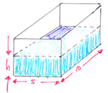
\includegraphics{images/diffeqns.png}
    \end{figure}

    Water in: $\frac{dV}{dt}=50$

    Water out: $\frac{dV}{dt}=-10h$

    Meaning that $\frac{dV}{dt}=50-10h$

    Volume of water in the cuboid: $V=50h$

    $\frac{dV}{dh}=50$

    $\frac{dV}{dt}=\frac{dV}{dh}\times \frac{dh}{dt}=50-10h$

    This means that $50\frac{dh}{dt}=50-10h$

    $5\frac{dh}{dt}=5-h$

    Separate variables and integrate:

    $\int \frac{5}{5-h}\,dh=\int dt$

    $-5\ln{|5-h|}=t+c$

    $\ln{|5-h|}=-\frac{t}{5}+C$

    $5-h=Ae^{-\frac{t}{5}}$

    $h=5-Ae^{-\frac{t}{5}}$

    When $t=0, h=2$:

    $2=5-A$

    $A=3$

    Model is: $h=5-3e^{-\frac{t}{5}}$

    To find how long it takes to get to a height of 4m:

    $4=5-3e^{-\frac{t}{5}}$

    $3e^{-\frac{t}{5}}=1$

    $e^{-\frac{t}{5}}=\frac{1}{3}$

    $-\frac{t}{5}=\ln{\frac{1}{3}}$

    $t=-5\ln{\frac{1}{3}}=5\ln{(\frac{1}{3})^{-1}}=5\ln{3}$ as required.


\end{enumerate}


\end{spacing}


\end{document}